\documentclass{standalone}
\usepackage{amsmath}
\usepackage{amssymb}
\usepackage{tikz}
\usepackage{mathrsfs}
\usepackage{ifthen}

\newcommand{\perpp}{\perp\!\!\!\perp}
\DeclareMathOperator{\so}{\mathfrak{s}}
\DeclareMathOperator{\ra}{\mathfrak{r}}
\DeclareMathOperator{\supp}{supp}
\DeclareMathOperator{\id}{id}
\DeclareMathOperator{\dom}{dom}
\DeclareMathOperator{\ran}{ran}
\DeclareMathOperator{\Min}{Min}
\DeclareMathOperator{\cod}{cod}
\newcommand{\smallerthan}{<}
\newcommand{\greaterthan}{>}
\newcommand{\defeq}{:=}
\newcommand{\eqdef}{=:}

\newcommand{\cat}[1]{\textbf{#1}}
\DeclareMathOperator{\IG}{\mathscr{IG}}


\begin{document}
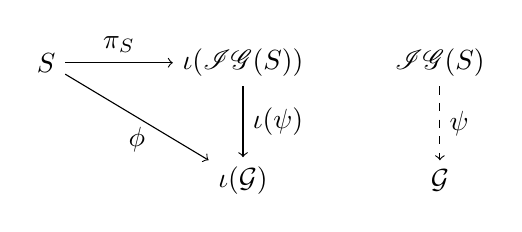
\begin{tikzpicture}
\node (S) at (0,0) {$S$};
\node (igS) at ([shift={+(2.5,0)}]S) {$\iota(\IG(S))$};
\node (iG) at ([shift={+(0,-1.5)}]igS) {$\iota(\mathcal{G})$};
\node (gS) at ([shift={+(2.5,0)}]igS) {$\IG(S)$};
\node (G) at ([shift={+(0,-1.5)}]gS) {$\mathcal{G}$};
\draw[->,dashed] (gS)--(G) node[right,midway] {$\psi$};
\draw[->] (igS)--(iG) node[right,midway] {$\iota(\psi)$};
\draw[->] (S)--(igS) node[above,midway] {$\pi_S$};
\draw[->] (S)--(iG) node[below,midway] {$\phi$};
\end{tikzpicture}\end{document}